\section{Limity równoległych zapytań}

\begin{figure}[!hb]
	\centering 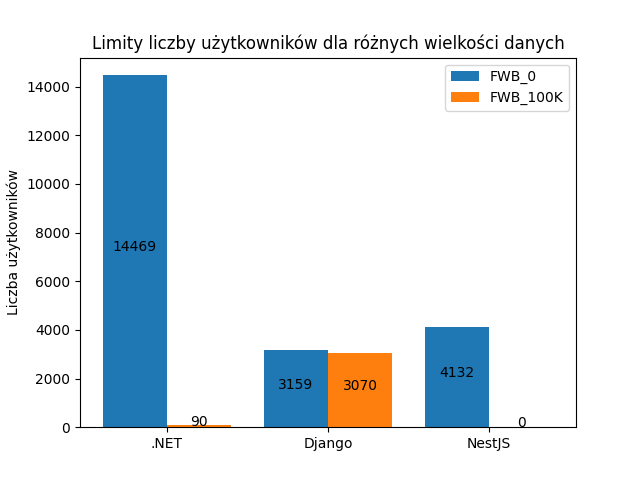
\includegraphics[width=1\linewidth]{rysunki/Limit_vus_for_different_datasets.png}
	\caption{Limit liczby użytkowników dla zwracajnych różnych wielkości danych dla jednej instacji frameworka}
	\label{rys:limit_vus}
\end{figure}

Django potrafi obsługiwać podobną ilość użytkowników dla obu zbiorów.
W przypadku zbioru danych FWB\_100K, narzędzie zanotowało spadek o niecałe 3\%.

Dotnet jest zdecydowanym liderem liczby użytkowników dla pustego zbioru. 
Widać u niego jednak znaczny spadek liczby obsługiwanych użytkowników wraz ze wzrostem ilości przesyłanych danych.

NestJS które przy zbiorze pustym jest nieco lepsze od Django, dla zbioru FWB\_100K całkowicie przestało odpowiadać - co oznacza, że nie radzi sobie z taką ilością danych.

